\subsection*{Divide and Conquer}
The problem is \textbf{divided} into smaller subproblems. If the subproblems are
large enough to be solved recursively, we call that the \textit{recursive case}.
Once the problem is too small, the recursion \textit{bottoms out} and we are at
the \textit{base case}. We can no longer recurse, and we solve the problem.
Sometimes the subproblems looks different than the original problem on top of
having to solve smaller instances of the same problem. This is the \textbf{conquer}
step. Lastly we \textbf{combine} the subsolutions and the original prolem is
solved.

\subsection*{Mergesort}
\textbf{Divide:} divides the sequence of size $n$ into two subsequence of size
$n/2$.\newline
\textbf{Conquer:} Sort the subsequences recursively until the sequences have
size $1$, in which case the subsequence is sorted.\newline
\textbf{Combine:} We merge the two sorted subsequences, making sure that they
appear in the correct order.
\newline\newline
The key operation in \texttt{Mergesort} is the combine step, where \texttt{Merge}
is called, since \texttt{Merge} merges two already sorted subsequences, and
ensures that the resulting merged sequence is sorted as well.

\subsubsection*{Example}
\begin{forest}
  for tree={
    draw,
    align=center
  }
  [$1$ $10$ $5$ $8$ $3$ $10$
    [$1$ $10$ $5$
      [$1$ $10$
        [$1$]
        [$10$]
      ]
      [$5$
        [$5$]
        [$\infty$]
      ]
    ]
    [$8$ $3$ $10$
      [$8$ $3$
        [$8$]
        [$3$]
      ]
      [$10$
        [$10$]
        [$\infty$]
      ]
    ]
  ]
\end{forest}
\newline\newline
\begin{forest}
  for tree={
    draw,
    align=center
  }
  [$1$ $3$ $5$ $8$ $10$ $10$
    [$1$ $5$ $10$ $\infty$
      [$1$ $10$ $\infty$
        [$1$ $\infty$]
        [$10$ $\infty$]
      ]
      [$5$ $\infty$
        [$5$ $\infty$]
        [$\infty$]
      ]
    ]
    [$3$ $8$ $10$ $\infty$
      [$3$ $8$ $\infty$
        [$8$ $\infty$]
        [$3$ $\infty$]
      ]
      [$10$ $\infty$
        [$10$ $\infty$]
        [$\infty$]
      ]
    ]
  ]
\end{forest}

$\infty$ is not in the final sequence since the last \texttt{for}-loop in
\texttt{Merge} only iterates for every element in the final sequence. That is
also why there is only one $\infty$ symbol for each subsequence.

\subsubsection*{Runtime $\Theta(n\log n)$}
The runtime of a \textbf{Divide-and-Conquer} algorithm is calculated as such:
\begin{align*}
  T(n)=
  \begin{cases}
    \Theta(n)&\textrm{ if }n\leq c\\
    aT(n/b)+D(n)+C(n)&\textrm{ otherwise.}
  \end{cases}
\end{align*}
\texttt{Merge} runs in $\Theta(n)$ time since at most $n$ basic steps are
performed. \texttt{Mergesort} find \textbf{divides} the problem by finding the
middle of the array. This happens in constant time. $D(n)=\Theta(1)$.
\newline\newline
Since the algorithm is \textbf{conquered} there are two recursive calls, each of
which represent half of the original problem, we have $2T(n/2)$.
\newline\newline
\texttt{Merge} \textbf{combines} the subsolutions. If \texttt{Merge} is called
with a sequence of size $n$, then $C(n)=\Theta(n)$.
\newline\newline
See recursion tree on the next page.
\begin{align*}
  T(n)=
  \begin{cases}
    \Theta(1)&\textrm{ if }n=1\\
    2T(n/2)+\Theta(n)&\textrm{ if }n>1.
  \end{cases}
\end{align*}
\begin{figure}[H]
  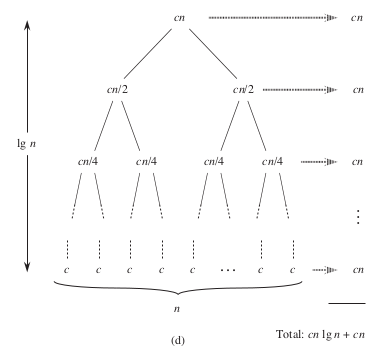
\includegraphics[scale=0.75]{pictures/recursiontree.png}
  \caption{Recursion tree of \texttt{Mergesort}}
\end{figure}
From the substitution tree, we can estimate that the runtime is
$\Theta(n\lg n-n)$. We shall now by substitution show if this holds.
\newline\newline
\textit{Guess:} $T(n)=O(n\lg n)$
\newline\newline
The want to find an upper bound on the recurrence
\begin{align*}
  T(n)=2T(\lfloor n/2\rfloor)+n
\end{align*}
We assume that this bound holds for $T(n)\leq cn\lg n\textrm{ for }n\geq n_0$.
We write:
\begin{align*}
  T(n)&\leq\textrm{ }2(c\lfloor n/2\rfloor\lg(\lfloor n/2\rfloor))+n&
  \textrm{Which is smaller than the assumed }T(n)\textrm{.}\\
  &\leq\textrm{ }cn\lg(n/2)+n\\
  &=\textrm{ }cn\lg n-cn\lg2+n\\
  &=\textrm{ }cn\lg-cn+n\\
  &\leq\textrm{ }cn\lg n\\\\
  T(n)&=
  \begin{cases}
    \Theta(1)&n=1\\
    \Theta(n\lg n)&n>1
  \end{cases}
\end{align*}
Via strong induction, we have proved the runtime.\newline\newline
\makecomment{The difference between weak induction and strong indcution only
appears in induction hypothesis. In weak induction, we only assume that
particular statement holds at k-th step, while in strong induction, we assume
that the particular statment holds at all the steps from the base case to k-th
step.}

\subsubsection*{Correctness: Proof by loop invariant}
In Mergesort the \textbf{combine} step solves the problem, and thus the
correctness of \texttt{Merge} will be proved.\newline\newline
We wish to maintain the following loop invariant:
\newline\newline
The \texttt{for}-loop loops from $k=p \texttt{ to } r$. Before each iteration of
the loop, we have the subsequence $A[p..k-1]$, which contains the $k-p$ smallest
elements of the sequences \texttt{L} and \texttt{R}. Furthermore $L[i]$ and
$R[j]$ are the smallest elements in the respective sequences that have not been
copied into \texttt{A}.
\newline\newline
\textit{Initialization:}\newline
Before the first iteration $k=p$ and therefore the $k-p=0$ smallest elements
have been added to $A[p..k-1]$, which then is empty. Since $i=j=1$, then $L[i]$
and $R[j]$ are the smallest elements in their respective sequences that have not
been copied into $A$.
\newline\newline
\textit{Maintenance:}\newline
There are two cases; $L[i]\leq R[j]$ and $L[i]<R[j]$.\newline\newline
$L[i]\leq R[j]$\newline
Before $L[i]$ is copied into $A$, then $A[p..k-1]$ contains the $k-p$ smallest
elements. After $L[i]$ is copied into $A$ it contains the $k-p+1$ smallest. $k$
and $i$ are incremented, and the loop invariant holds before the next iteration.
\newline\newline
$L[i]>R[j]$\newline
Here $R[j]$ is added to the $A$, and $k$ and $j$ are incremented. The loop
invariant also holds for this case.
\newline\newline
\textit{Termination:}\newline
The loop terminates when $k=r+1$, since $r$ is the last element in $A[p..r]$,
where $r=k-1$. $A$ now contains the $k-p=r-p+1$ smallest elements of $L$ and
$R$. Only the largest element of both $L$ and $R$ have been added since the
largest element of each array is a sentinel ($\infty$). The loop invariant holds.
